\documentclass[12pt]{article}
%\usepackage[utf8]{inputenc}
%\documentclass[UTF8]{ctexart}
%\usepackage[UTF8, heading = false, scheme = plain]{ctex}
\usepackage{geometry}
%geometry{a4paper,scale=0.9}
\geometry{a4paper,left=1cm,right=1cm,top=1cm,bottom=2cm}
\usepackage{amsfonts}
\usepackage{color}
\usepackage{url}
%\usepackage{biblatex}
\usepackage{amsmath}
\usepackage{amssymb}
\usepackage{latexsym}
\usepackage{cite}
%\addbibresource{ref.bib}
%\bibliography{ref.bib}
\usepackage{caption}
\usepackage{graphicx, subfig}
\usepackage{float}
%\usepackage[fontset=ubuntu]{ctex}
%\usepackage{fontspec}
\usepackage{xeCJK}
%\usepackage[colorlinks,
%anchorcolor=black,
%citecolor=black]{hyperref}
%\setmainfont{SimSun}
\usepackage[section]{placeins}
\usepackage{enumitem}
\usepackage{framed}
\usepackage[framemethod=TikZ]{mdframed}
\usepackage{indentfirst}
\usepackage{setspace}%使用间距宏包
\linespread{1.5}

\title{信息论\cite{InfomationTheory_Example_Poison}}
%\author{leolinuxer }
%\date{June 2020}


\begin{document}
%\setlength{\parindent}{0pt}
\maketitle
\tableofcontents

\section{信息熵}
\subsection{热力学中的熵}
熵的概念最早起源于物理学,用于度量一个热力学系统的无序程度,也就是系统混乱程序。

熵增定律指出:在一个孤立系统里,如果没有外力做功,其总混乱度(熵)会不断增大。

\subsection{信息论中的熵}
在信息论中,熵的概念和热力学中是类似的,描述的是“信息的不确定程度”。

\begin{itemize}[itemindent=2em]
    \item 热力学熵:\textbf{系统的混乱程度}
    
    \item 信息熵:\textbf{信息的不确定性的度量}
\end{itemize}

所以信息中的不确定性类似于热力学中系统的混乱程度。也就是说,信息的不确定程度越大,信息熵也就越大。那什么样的信息不确定程度大呢?

比如抛一枚硬币,如果我来猜正反的话,那么我基本只能靠瞎蒙,因为不确定程度很大,正反的概率都是 0.5。对于抛一次硬币猜正反这类事件来说,它的不确定程度很大,信息熵也很大。

如果中国男足和巴西男足比赛,让我来猜胜负,那么我几乎可以断言,巴西队一定会赢。也就是巴西队和中国队胜负这个事件的不确定程度很小,信息熵也就很小。如果比赛前我告诉你一条信息“巴西队肯定会赢“,那么这条信息的信息量几乎为零,因为这条信息并没有降低信息的不确定度。

\subsection{信息、信息熵、信息量的关系}
上面提到了信息熵、信息、信息量,它们之间的比较如下:

\begin{itemize}[itemindent=2em]
    \item 凡是在一种情况下能减少不确定性的任何事物都叫\textbf{信息},否则叫作废话。比如经常会碰到有人絮絮叨叨,不知所云,说了好久不知道要表达什么。从信息论的角度来看,这些话就不包含信息。
    
    \item \textbf{信息熵}是一个绝对值,用来衡量信息不确定程度的绝对大小。
    
    \item \textbf{信息量}是一个相对值,表示的是在给出一条信息后,信息熵前后的减小值。如果信息熵减小的越大,说明这条信息的信息量越大。比如福彩 35 选 7,如果有人直接告诉你这 7 个数字,那么这条信息的信息量就超级大,因为它直接将信息熵降为 0。
\end{itemize}

\subsection{信息熵的定量表述}
香农把随机变量$X$的熵值 $Η$ 定义如下:
$$H(X) = -\sum_i{P(x_i)\log_bP(x_i)}$$

$b$ 是对数所使用的底。当$b=2$,熵的单位是bit。

$P$ 为$X$的概率质量函数(probability mass function),我们可以理解为事件 $x_i$ 发生的概率。

公式看起来可怕,其实非常简单。让我们用抛硬币来举例,“抛一次硬币得到正面或者反面”这个随机变量 $X$ 的信息熵为:
$$H(X) = -(\frac{1}{2}\log_2{\frac{1}{2}}+\frac{1}{2}\log_2{\frac{1}{2}}) = -\log_2{\frac{1}{2}} = 1 $$

也就是抛一次硬币是正面还是反面这个事件的信息熵只需要 1 bit,也就是只需要用 1 位的二进制数就可以表示这个信息大小。也就是说,在计算机中,我们给抛硬币这个事件进行编码,只需要1个bit的信息就可以描述了,比如 0 带代表反面,1代表正面。

\section{信息论的一个例子}
\textbf{1000桶水,其中一桶有毒,猪喝毒水后会在15分钟内死去,想用一个小时找到这桶毒水,至少需要几头猪?}

这道题看起来像是一道算法题,本质上却是披着羊皮的信息论问题。解答这道题并不是我的目的,我的目的是用信息论的思维来思考,达到触类旁通,一通百通。

用信息论去思考的另一个好处就是,{\color{red}{信息论给了这类问题的一个边界,让我们在边界范围内思考问题}}。很难想象,70多年前的香农已经用严格的理论证明为这类问题设定了一个极限,任何想逾越这个极限去解决问题的人最后都会被证明是徒劳的。

这也是理论武装头脑的好处,当别人还在尝试是否有更优的解法时,你可以直接给出最优答案,用信息论降维打击。即使我可能暂时无法想出具体的方案,但我知道这类问题的一个理论极限在哪里,没有必要为超越极限做无用功。

\subsection{题目的简化版本}

在我们学习了信息熵的知识以后,让我们再来看题目。原题其实略微复杂一些,先将题目简化一下:1000 桶水,其中一桶有毒,猪喝毒水后会在 15 分钟内死去,想用 15 分钟内找到这桶毒水,至少需要几头猪?

首先,“1000 桶水其中有一桶有毒”可以用随机变量 $X$ 来描述($X=i$ 表示第$i$桶水有毒),那么这个随机变量 X 的信息熵为:
$$
H(X) = -\sum_i^{N}P(X_i)\log_2{P(X_i)} = -\sum^{1000}\frac{1}{1000}\log_2{\frac{1}{1000 }} = -\log_2{\frac{1}{1000}} = 9.966
$$

也就是说,在计算机中,我们给“哪通水有毒”这个事件进行编码,只需要10个bit的信息就可以描述了,比如 0000000001 代表第一桶水有毒。

1 只猪喝水以后的要么活着,要么死去,一共有两种状态,所以”1 只猪喝完水以后的状态“这个随机变量 Y 的信息熵为
$$H(Z) = -(\frac{1}{2}\log_2{\frac{1}{2}}+\frac{1}{2}\log_2{\frac{1}{2}}) = -\log_2{\frac{1}{2}} = 1$$

n 只猪喝完水会有$2^n$种状态,即"n 只猪喝完水以后的状态"这个随机变量 $Y$ 的信息熵为:
$$H(Y) = \sum_{i=1}^{2^n}P(y_i)I(y_i)=-\sum_{i=1}^{2^n}\frac{1}{2^n}\log_2{\frac{1}{2^n}} = -\log_2{\frac{1}{2^n}} = n$$

所以,按照题目要求,如果至少需要 n 头猪能够找到这桶毒水,那么随机变量 $Y$ 的信息熵必须要大于随机变量 $X$ 的信息熵,也就是 $H(Y)>=H(X)$,即$n>=9.966$,所以 $n=10$。

其实,上面的信息熵计算的简化版本可以写成如下更好理解的形式:
$$2^n>=1000$$

同样可以解得 $n = 10$ ,虽然形式简单,但我们一定要记住它背后的原理是信息熵。

\subsection{简化后题目的具体方案}
\begin{figure}[ht]
  \centering
  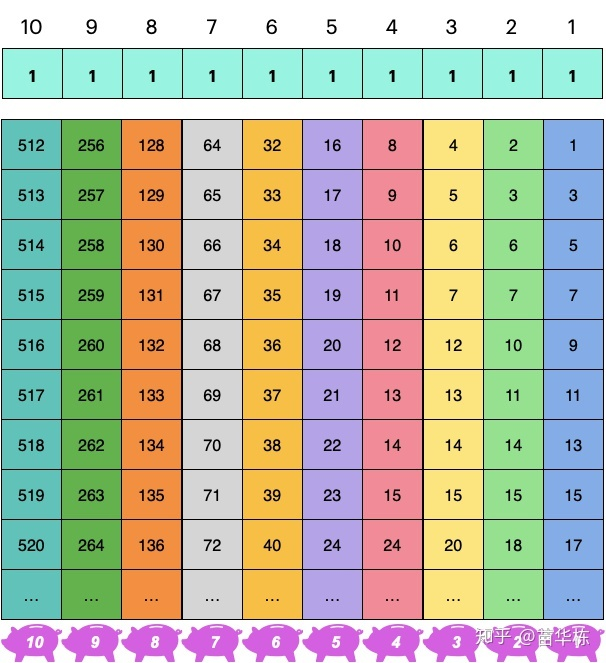
\includegraphics[width=.5\textwidth]{fig/InfomationTheory_Poison_Encode.jpg} %1.png是图片文件的相对路径
  \caption{编码方式} %caption是图片的标题
  \label{InfomationTheory_Poison_Encode} %此处的label相当于一个图片的专属标志,目的是方便上下文的引用
\end{figure}
我们将 1000 桶水按照 2 进制编码,如图第一行,需要 10 位二进制数。于是有

\begin{itemize}[itemindent=2em]
    \item 第 1 桶水对应上图最右侧位置 1 的数字是 1,其它数字都是 0,也就是 00000 00001b,其中 b 代表二进制数。
    
    \item 第 10 桶水对应上图位置 4 和位置 2 的数字是 1,其它数字都是 0,也就是 00000 01010b。
    
    \item 同理,任意一桶水,都可以对应上面唯一的一个二进制数。
\end{itemize}

于是,我按照如下方案让猪进行喝水,如上图所示:

\begin{itemize}[itemindent=2em]
    \item 1 号猪喝位置 1 的数字是 1 的水,也就是 1、3、5、7、9 ...
    
    \item 2 号猪喝位置 2 的数字是 1 的水,也就是 2、3、6、7、10 ...
    
    \item ……
\end{itemize}

如果 15 分钟后 1,3,5 号猪被毒死,那么对应的二进制编码就是 00000 10101b,也就是 21 号水桶有毒。更一般的,猪死的任何一种排列方式都对应了二进制的唯一编码。

\subsection{原题目}
1000 桶水,其中一桶有毒,\textbf{猪喝毒水后会在 15 分钟内死去,想用一个小时找到这桶毒水},至少需要几头猪?

有了前面简化的版本的理解,我们容易得知

”1000 桶水其中有一桶有毒“这个随机变量 X 的信息熵为:
$$H(X)=-\log_2{\frac{1}{1000}} = 9.966$$

而对于猪的状态就不太一样了,我们可以想象一下,一只猪在一个小时内会有几种状态?
\begin{itemize}[itemindent=2em]
    \item 在第 0 分钟的时候喝了一桶水以后,第 15 分钟死去。
    
    \item 第 15 分钟依然活着,喝了一桶水以后,第 30 分钟死去。
    
    \item 第 30 分钟依然活着,喝了一桶水以后,第 45 分钟死去。
    
    \item 第 45 分钟依然活着,喝了一桶水以后,第 60 分钟死去。
    
    \item 第 45 分钟依然活着,喝了一桶水以后,第 60 分钟依然活着。
\end{itemize}

可见,1 只猪 1 个小时以后会有 5 种状态,所以”1 只猪 1 个小时后的状态“这个随机变量 $Z$ 的信息熵为:
$$H(Z) = -(5\times\frac{1}{5}\log_2{\frac{1}{5}}) = \log_2{5} = 2.3219$$

n 只猪 1 个小时后会有 $5^n$ 种状态,即"n 只猪 1 个小时以后的状态"这个随机变量 $Y$ 的信息熵为:
$$H(Y) = \sum_{i=1}^{5^n}P(y_i)I(y_i)=-\sum_{i=1}^{5^n}\frac{1}{5^n}\log_2{\frac{1}{5^n}} = -\log_2{\frac{1}{5^n}} = n\log_2{5} = 2.3219n$$

所以,按照题目要求,如果至少需要 n 头猪能够找到这桶毒水,那么随机变量 $Y$ 的信息熵必须要大于随机变量 $X$ 的信息熵,也就是:
$H(Y)>=H(X)$,即$n>=9.966/2.3219=4.292$,所以 $n=5$。

事实上,对于 n = 5 来说,不仅可以检测 1000 桶水,甚至检测 3000 桶水都是没有问题的。有兴趣的童鞋可以试着计算一下。

到此,香农给了我们一个理论极限,但是具体的方案还是需要我们自己进行构造。得出 n=5 是依靠我们的理论功底,而得出具体的方案就是我们的工程水平了。

根据前面简化版本的二进制编码方式的思路,我们是不是可以利用猪的 5 种状态构造一个 5 进制编码方式呢?如下图所示。

\begin{figure}[ht]
	\centering  %图片全局居中
	\subfloat[第一张] %第一张子图
    {
        \begin{minipage}[t]{0.8\textwidth}
            \centering          %子图居中
            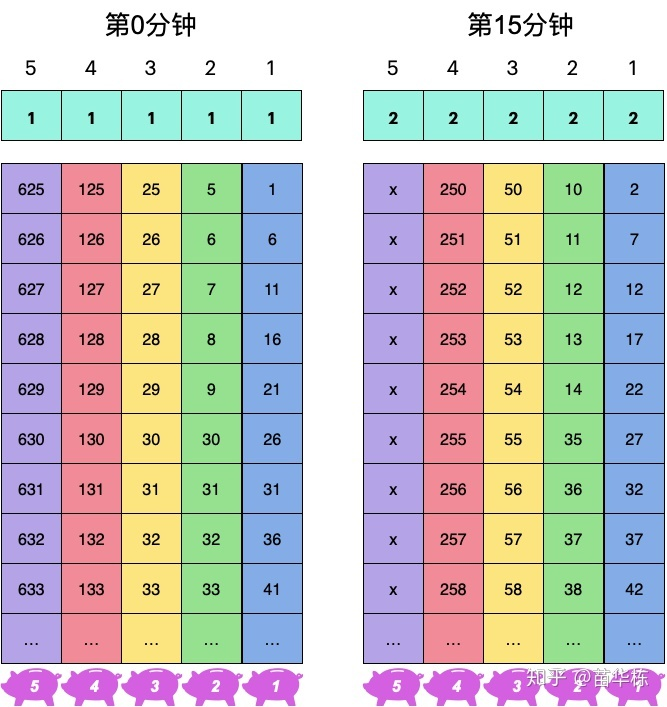
\includegraphics[width=0.5\textwidth]{fig/InformationTheory_Poison_Encode_5_1.jpg}   %以行宽的0.5倍大小显示
        \end{minipage}%
    }%注意这里回车空行后两张图会上下排列,否则会并排排列
    
    \subfloat[第二章] %第二张子图
    {
        \begin{minipage}[t]{0.8\textwidth}
            \centering      %子图居中
            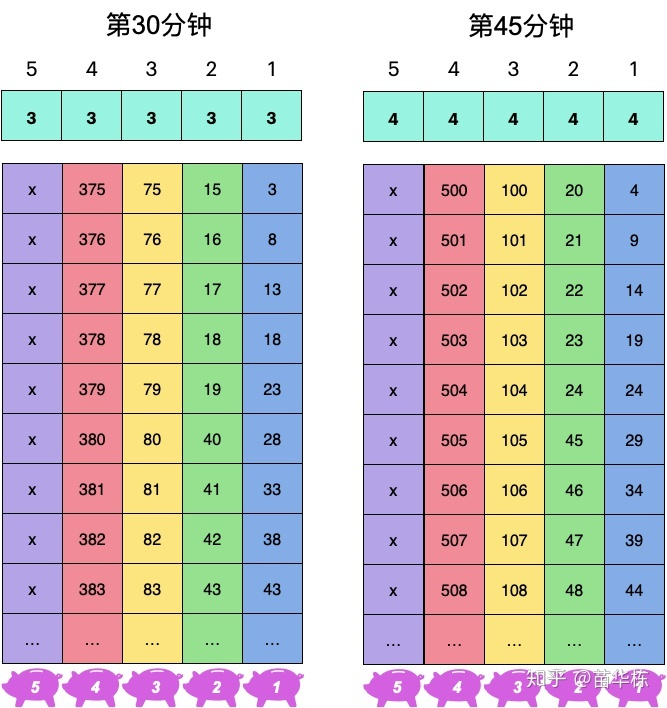
\includegraphics[width=0.5\textwidth]{fig/InformationTheory_Poison_Encode_5_2.jpg}   %以行宽的0.5倍大小显示
        \end{minipage}
    }%
	\caption{编码方式}
	\label{level}
\end{figure}


首先,将 1000 桶水按照 5 进制编码的方式排列,如上图所示,需要 5 位 5 进制数。然后按照如下方案让猪进行喝水,如上图所示:
\begin{itemize}[itemindent=2em]
    \item 1 号猪第 0 分钟喝位置 1 的数字是 1 的水,如图所示,也就是 1、6、11、16、21...
    
    \item 如果第 15 分钟活着,喝位置 1 的数字是 2 的水,如图所示,也就是 2、7、12、17、22...
    
    \item 如果第 30 分钟活着,喝位置 1 的数字是 3 的水,如图所示,也就是 3、8、13、18、23...
    
    \item 如果第 45 分钟活着,喝位置 1 的数字是 4 的水,如图所示,也就是 4、9、14、19、24...
    
    \item 类似的,2 号猪喝位置 2 的水...
\end{itemize}

上面,猪的编号代表 5 进制编码数字所在的位数,1 号猪代表最末位,5 号猪代表最高位。而第几分钟死代表当前位数的权重,15 分钟死表示权重是 1,30 分钟死表示权重是 2,... ,60 分钟死表示权重是 4,60 分钟依然活着表示权重是 0。

如果 1 号猪第 30 分钟死了,2 号猪第 15 分钟死了,3 号猪第 45 分钟死了,4,5 号都活到了最后。则毒水对应的 5 进制编码是
$$0\times5^4+0\times5^3+3\times5^3+1\times5^2+2\times5^0=82$$

也就是第 82 桶水有毒。

%\printbibliography
\bibliography{../ref}
\bibliographystyle{IEEEtran}
\end{document}